\section{Chapter three}

\vspace*{\fill}

\begin{example}
  \centering
  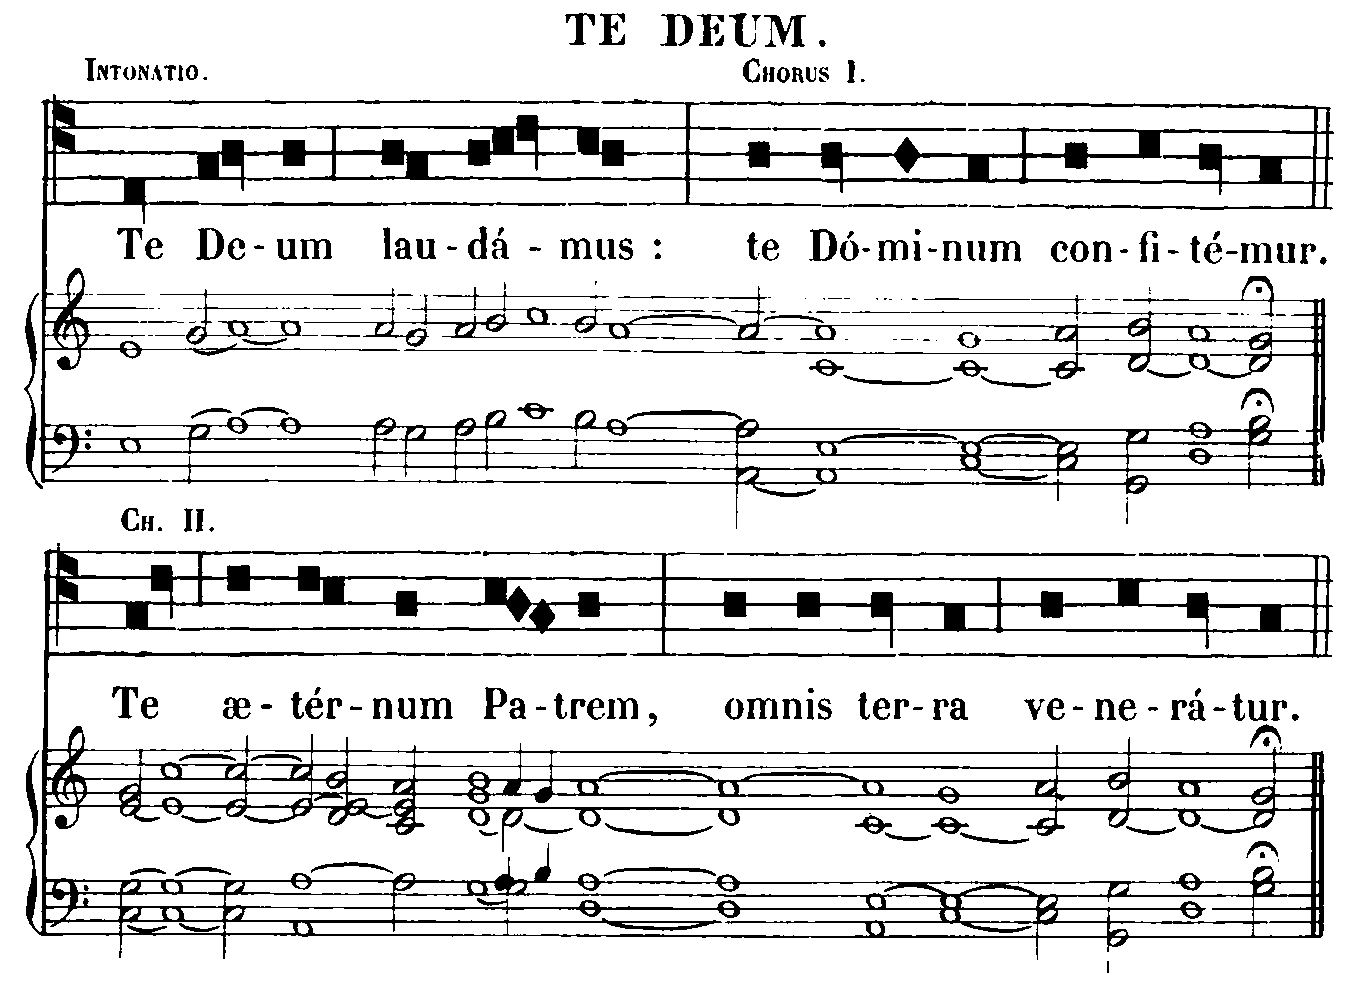
\includegraphics[width=\linewidth]{c/3/ex/gevaert_vademecum.png}
  \caption{Gevaert, Hexachordal accompaniment, 1871}
  \label{mus:gevaert_vademecum}
\end{example}

\vspace*{\fill}

\newpage

\vspace*{\fill}

\begin{example}
  \centering
  \includegraphics[width=.8\linewidth]{c/3/ex/vandamme_pange.png}
  \caption{Van Damme, Modulating interlude, \emph{c}.1870s}
  \label{mus:vandamme_pange}
\end{example}

\vspace*{\fill}

\newpage

\vspace*{\fill}

\begin{example}
  \centering
  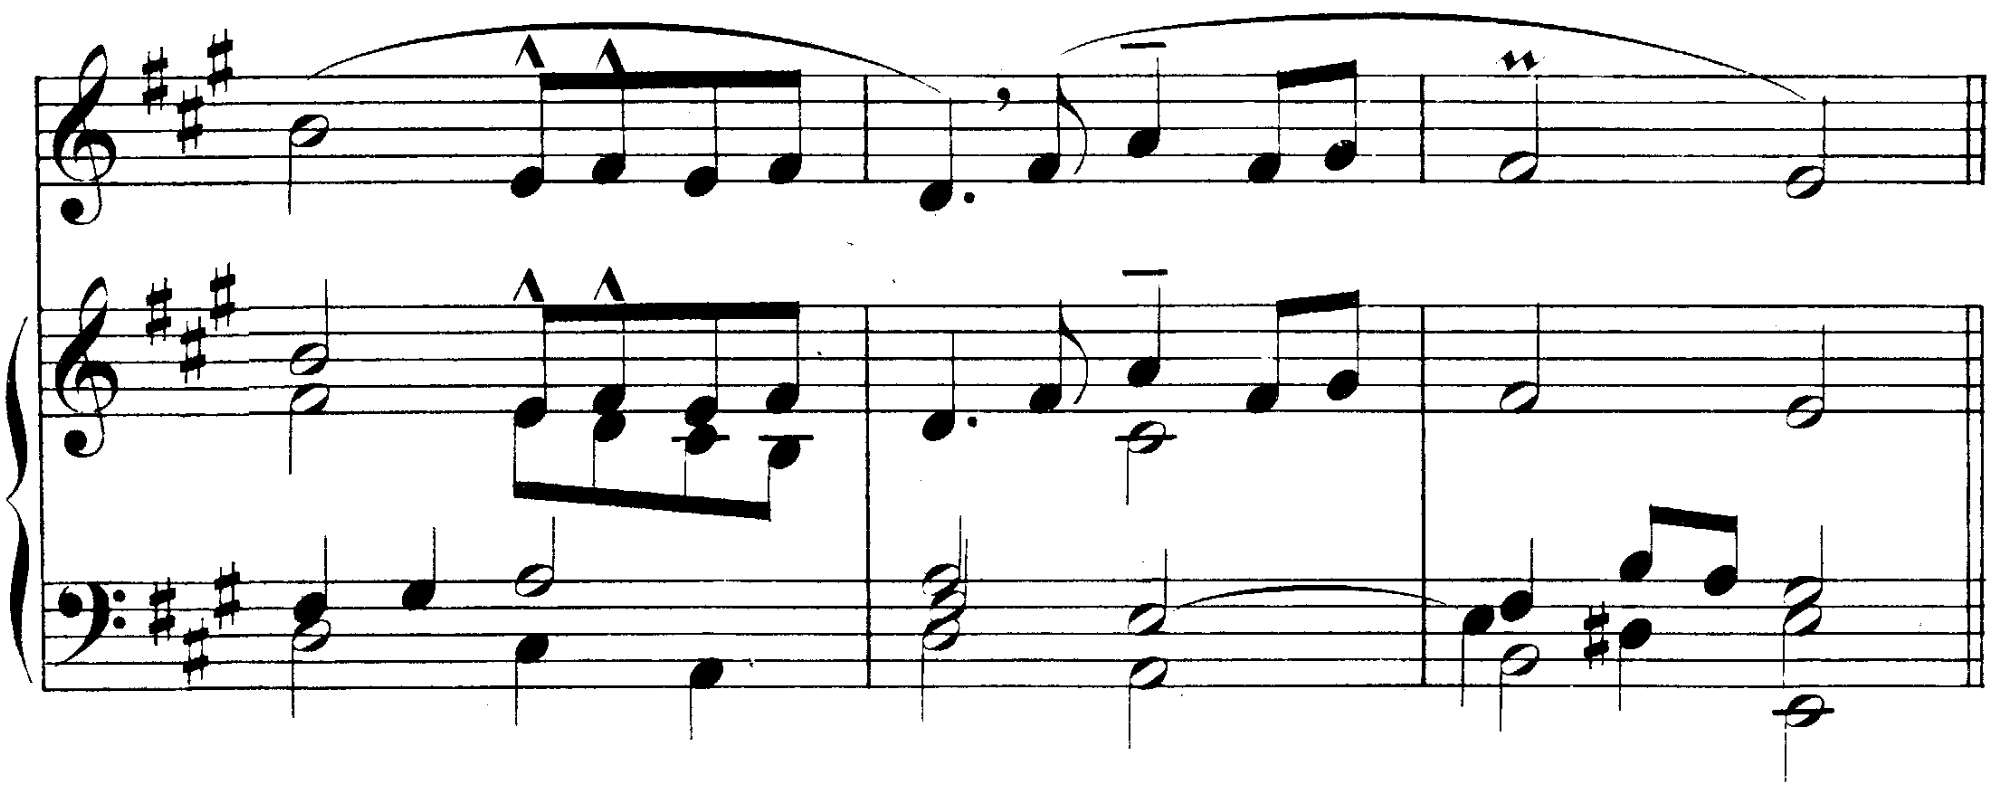
\includegraphics[width=.8\linewidth]{{c/3/ex/lemmens_sharp.png}}
  \caption{Lemmens, Sharped cadence, 1884}
  \label{mus:lemmens_sharped}
\end{example}

\vspace*{\fill}

\begin{example}
  \centering
  \includegraphics[width=.9\linewidth]{{c/3/ex/lemmens_nosharp.png}}
  \caption{Lemmens, Diatonic cadence, 1884}
  \label{mus:lemmens_nosharped}
\end{example}

\vspace*{\fill}

\newpage

\vspace*{\fill}

\begin{example}
  \centering
  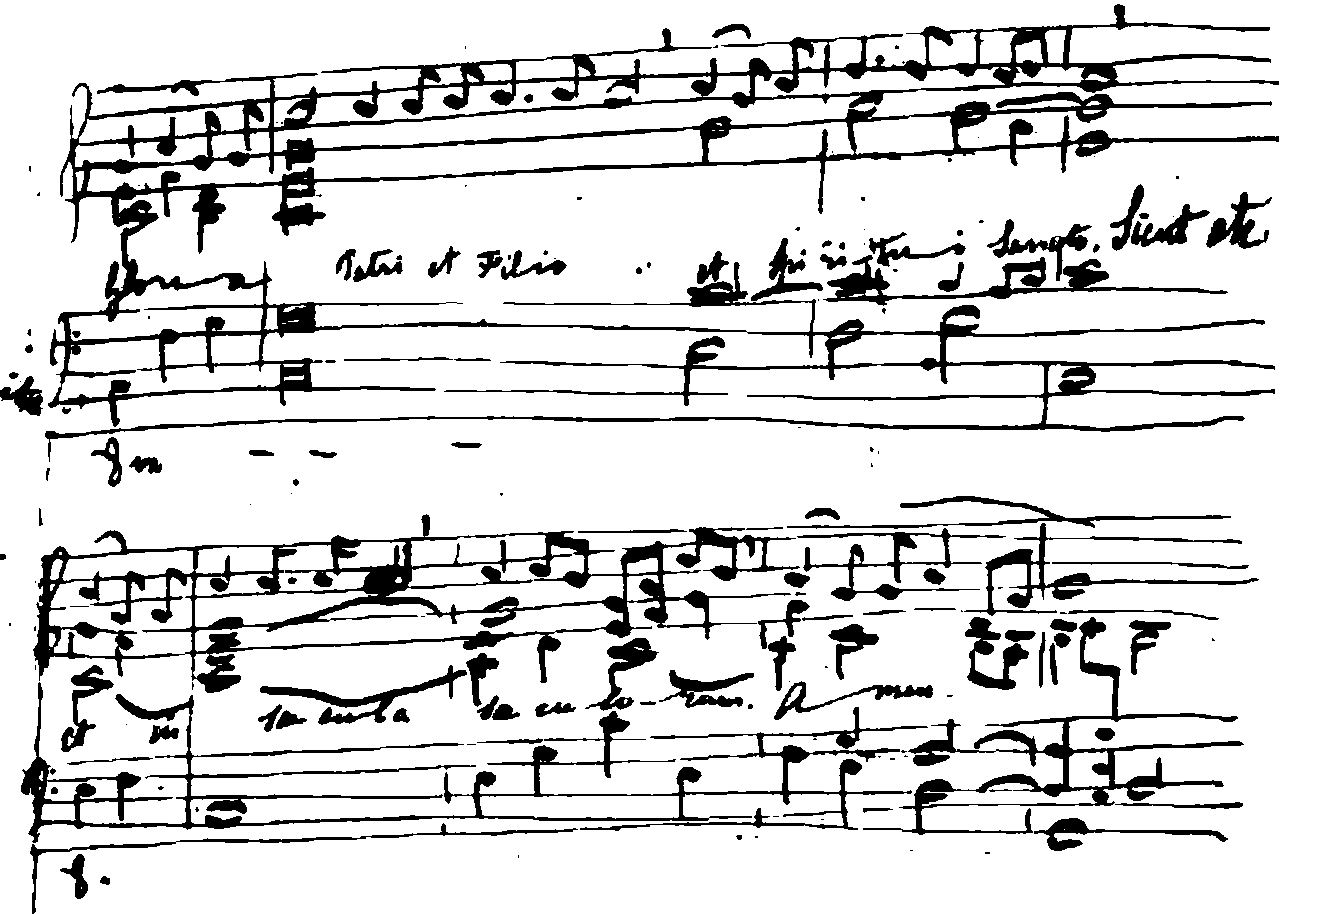
\includegraphics[width=\linewidth]{c/3/ex/lemmens_pothier.png}
  \caption{Lemmens to Pothier, Mensurated accompaniment, 21 December 1879}
  \label{mus:lemmens_pothier}
\end{example}

\vspace*{\fill}

\begin{example}
  \centering
  \includegraphics[width=\linewidth]{c/3/ex/vandamme_requiem.png}
  \caption{Van Damme, `Kyrie' from \emph{Missa pro defunctis}, 1881}
  \label{mus:vandamme_requiem}
\end{example}

\vspace*{\fill}

\newpage

\vspace*{\fill}

\begin{example}
  \centering
  \includegraphics[width=.8\linewidth]{c/3/ex/vandammepothier.png}
  \caption{Van Damme, Early instance of filled-and-void notation}
  \label{mus:vandammepothier}
\end{example}

\vspace*{\fill}

\newpage

\vspace*{\fill}

\begin{example}
  \centering
  \includegraphics[width=\linewidth]{c/3/ex/vandamme_ordinarium.png}
  \caption{Van Damme, \emph{Ordinarium Miss\ae{}} with filled-and-void notation, 1884}
  \label{mus:vandamme_ordinarium}
\end{example}

\vspace*{\fill}

\begin{example}
  \centering
  \includegraphics[width=.9\linewidth]{{c/3/ex/vandamme_vespers.png}}
  \caption{Van Damme, Cross showing metrical accent, 1885}
  \label{mus:vandamme_vespers}
\end{example}

\vspace*{\fill}

\begin{example}
  \centering
  \includegraphics[width=\linewidth]{c/3/ex/oblique_1907.png}
  \caption{Near-horizontal oblique, \emph{c}.1907}
  \label{mus:oblique_1907}
\end{example}

\vspace*{\fill}

\begin{landscape}

  \vspace*{\fill}

  \begin{example}
    \centering
    \includegraphics[width=.8\linewidth]{c/3/ex/schmetzpiel_ord_51.png}
    \caption{Piel and Schmetz, Extract from \emph{Ordinarium miss\ae{}}, \emph{c}.1886}
    \label{mus:schmetzpiel_ord_51}
  \end{example}

  \vspace*{\fill}

\end{landscape}

\vspace*{\fill}

\begin{example}
  \centering
  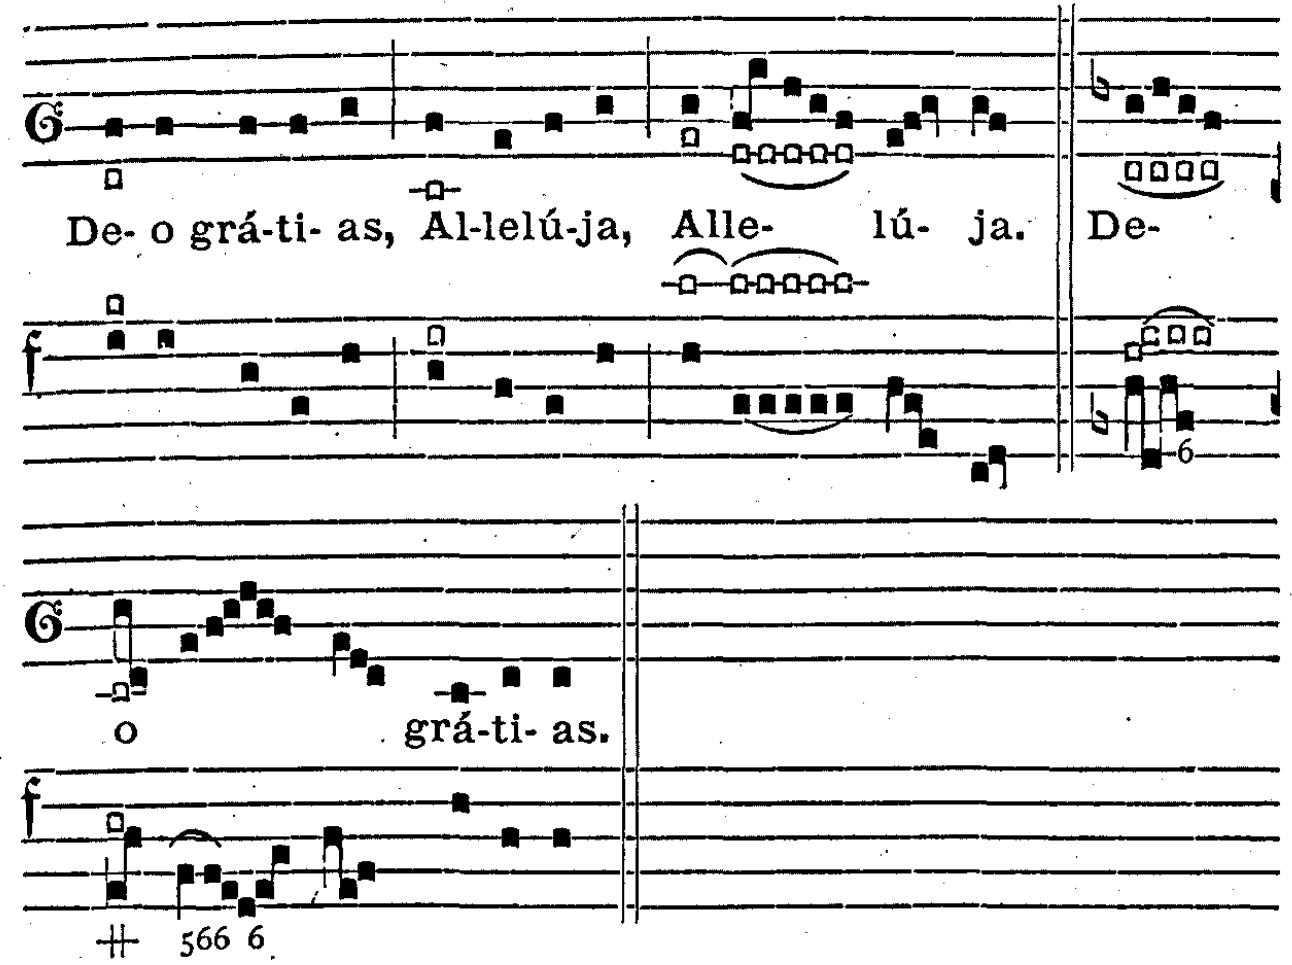
\includegraphics[width=.8\linewidth]{c/3/ex/schmetz_deogratias_35.png}
  \caption{Schmetz--Piel, Harmonic quadratic notation, 1884}
  \label{mus:schmetz_deogratias_35}
\end{example}

\vspace*{\fill}

\begin{example}
  \includely[nofragment,staffsize=14]{c/3/ex/schmetz/schmetz}
  \caption{Realisation of \cref{mus:schmetz_deogratias_35}}
  \label{mus:schmetz_transcription}
\end{example}

\vspace*{\fill}

\clearpage
\vspace*{\fill}
\begin{example}
  \centering
  \includegraphics[width=.8\linewidth]{c/3/ex/pothier_christe_7star.png}
  \caption{Pothier, `Christe' from \emph{In Festis Solemnibus I}, 1883}
  \label{mus:pothier_christe_7star}
\end{example}
\vspace*{\fill}
\begin{example}
  \centering
  \includegraphics[width=\linewidth]{c/3/ex/schmetz_christe_59.png}
  \caption{Schmetz, Applying \emph{Liber gradualis} neumes, 1885}
  \label{mus:schmetz_christe_59}
\end{example}
\vspace*{\fill}
\clearpage

%%%%%%%%%%%%%%%%%%%%%%%%%%%%%%%%%%%%%%%%%%%%%%%%%%%
%                                                 %
%                  SECTION TWO                    %
%                                                 %
%%%%%%%%%%%%%%%%%%%%%%%%%%%%%%%%%%%%%%%%%%%%%%%%%%%

\vspace*{\fill}

\begin{example}
  \centering
  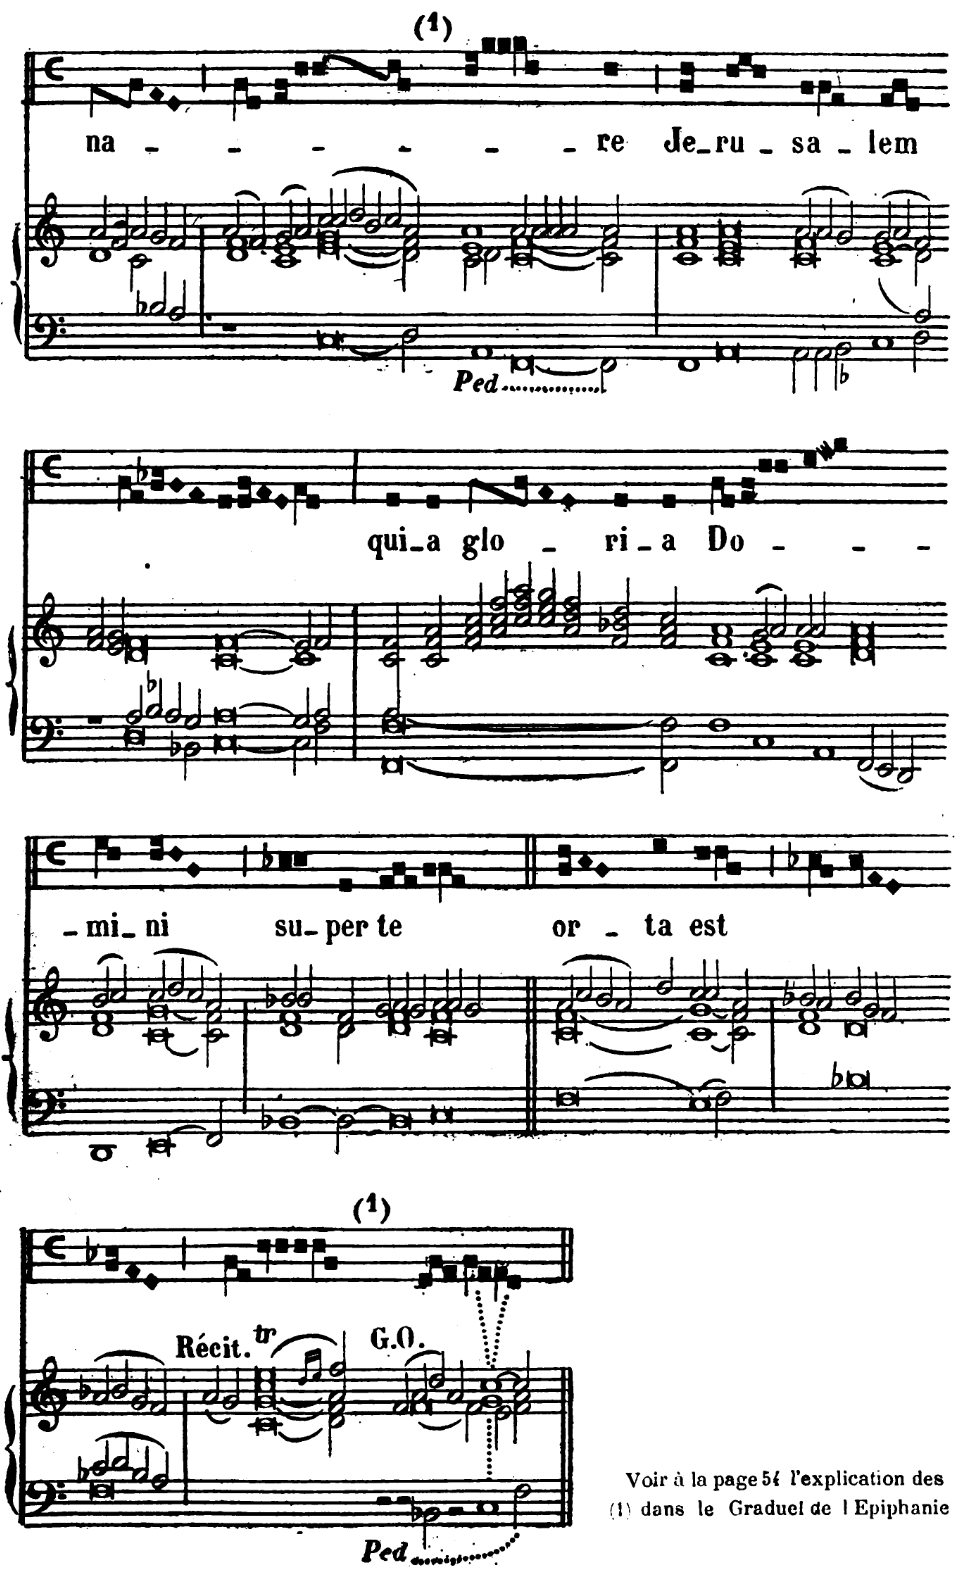
\includegraphics[width=.7\linewidth]{c/3/ex/lhoumeau_epiphany_53.png}
  \caption{Lhoumeau, Instrumental accompaniment, 1884}
  \label{mus:lhoumeau_epiphany_53}
\end{example}

\vspace*{\fill}

\clearpage

\vspace*{\fill}

\begin{example}
  \centering
  \includegraphics[width=.9\linewidth]{c/3/ex/lhoumeau_syllabic.png}
  \caption{Lhoumeau, Chords changing on \emph{theses}, 1892}
  \label{mus:lhoumeau_syllabic}
\end{example}

\vspace*{\fill}

\begin{example}
  \centering
  \includegraphics[width=.6\linewidth]{c/3/ex/lhoumeau_torculus.png}
  \caption{Lhoumeau, Bass notes changing on final neumatic note, 1893}
  \label{mus:lhoumeau_torculus}
\end{example}

\vspace*{\fill}

\clearpage

\vspace*{\fill}

\begin{example}
  \centering
  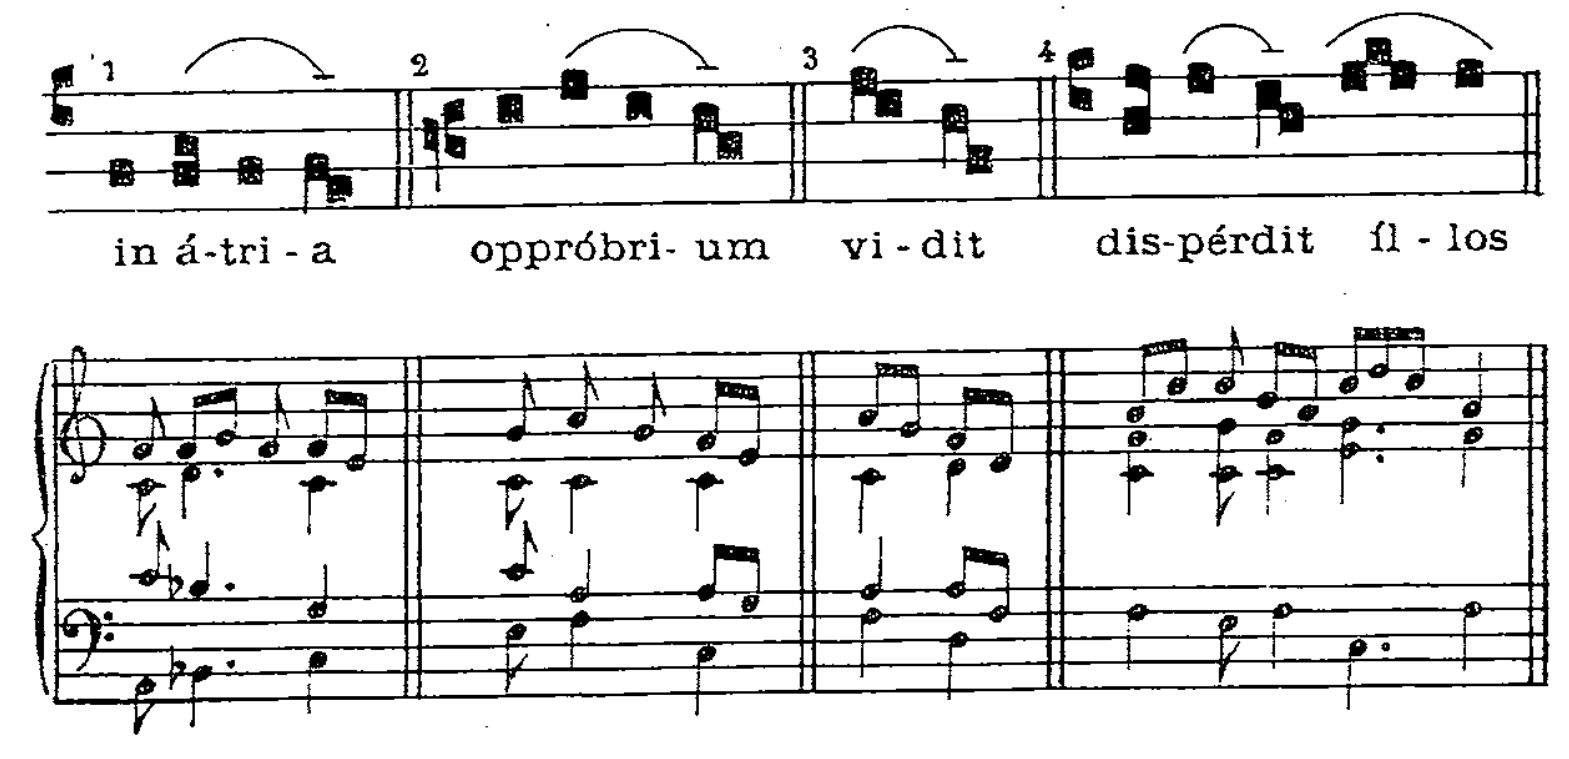
\includegraphics[width=\linewidth]{c/3/ex/lhoumeau_feminine.png}
  \caption{Lhoumeau, Feminine endings, 1892}
  \label{mus:lhoumeau_feminine}
\end{example}

\vspace*{\fill}

\begin{example}
  \centering
  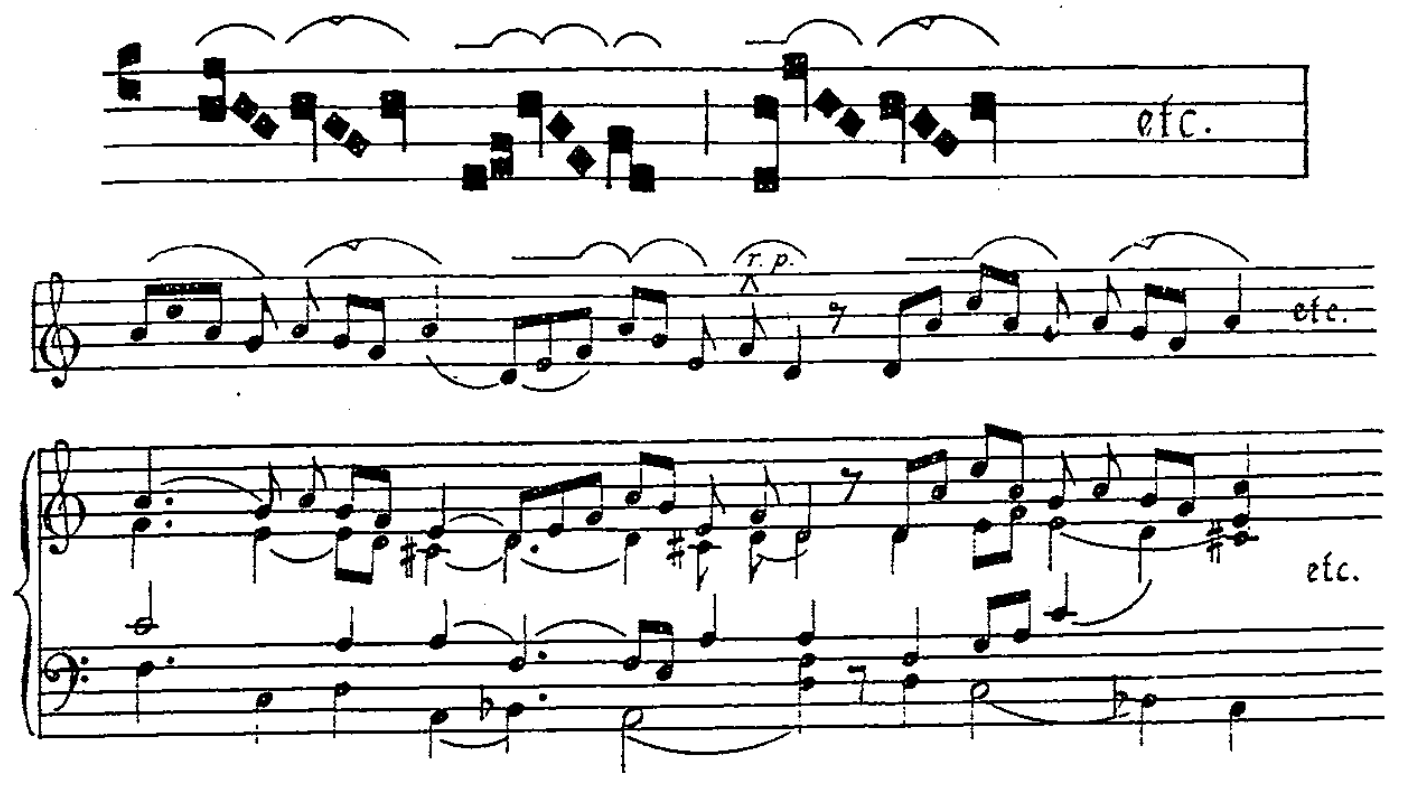
\includegraphics[width=\linewidth]{c/3/ex/lhoumeau_alleluia.png}
  \caption{Lhoumeau, Melismatic accompaniment, 1892}
  \label{mus:lhoumeau_alleluia}
\end{example}

\vspace*{\fill}

\clearpage

\begin{landscape}
  \vspace*{\fill}
  \begin{example}
    \centering
    \includegraphics[width=.8\linewidth]{c/3/ex/clement_awkward_191.jpg}
    \caption{Clément, Awkward voice leading, 1894}
    \label{mus:clement_awkward_191}
  \end{example}
  \vspace*{\fill}
\end{landscape}

\vspace*{\fill}

\begin{example}
  \includely[nofragment,staffsize=14]{c/3/ex/teppe/gigoutone}
  \caption{Gigout, Sustained harmonisation according to Teppe's rhythm, 1889}
  \label{mus:teppe_gigoutone}
\end{example}

\vspace*{\fill}


\begin{example}
  \includely[nofragment,staffsize=14]{c/3/ex/teppe/gigouttwo}
  \caption{Gigout, Instrumental harmonisation according to Teppe's rhythm, 1889}
  \label{mus:teppe_gigouttwo}
\end{example}


\vspace*{\fill}

\clearpage

\vspace*{\fill}

\begin{example}
  \centering
  \includegraphics[width=\linewidth]{c/3/ex/gigout_1_5.jpg}
  \caption{Gigout, Unaccompanied notes, 1892}
  \label{mus:gigout_1_5}
\end{example}

\vspace*{\fill}

\begin{example}
  \centering
  \includegraphics[width=\linewidth]{c/3/ex/gigout_2_7.jpg}
  \caption{Gigout, Chord-against-note style, 1892}
  \label{mus:gigout_2_7}
\end{example}

\vspace*{\fill}

\clearpage

\vspace*{\fill}

\begin{example}
  \centering
  \includegraphics[width=\linewidth]{c/3/ex/gigout_4_20.png}
  \caption{Gigout, `Più lento' style, 1892}
  \label{mus:gigout_4_20}
\end{example}

\vspace*{\fill}

\begin{example}
  \centering
  \includegraphics[width=\linewidth]{c/3/ex/boellmann_3_7.png}
  \caption{Boëllmann, Similar approach to \cref{mus:gigout_4_20} but for rests, 1892}
  \label{mus:boellmann_3_7}
\end{example}

\vspace*{\fill}

\clearpage

\vspace*{\fill}

\begin{example}
  \centering
  \includegraphics[width=\linewidth]{c/3/ex/gounod_3_18.jpg}
  \caption{Gounod, Chord-against-note style, 1892}
  \label{mus:gounod_3_18}
\end{example}

\vspace*{\fill}

\begin{example}
  \centering
  \includegraphics[width=\linewidth]{c/3/ex/widor_2_1.jpg}
  \caption{Widor, Chord-against-note style, 1892}
  \label{mus:widor_2_1}
\end{example}

\vspace*{\fill}

\clearpage

\vspace*{\fill}

\begin{example}
  \centering
  \includegraphics[width=\linewidth]{c/3/ex/tinel_4_2.png}
  \caption{Tinel, Obliques and accompaniment in two or three parts, 1892}
  \label{mus:tinel_4_2}
\end{example}

\vspace*{\fill}

\begin{example}
  \centering
  \includegraphics[width=\linewidth]{c/3/ex/busschaert_4_11.png}
  \caption{Busschaert, Rests as blank space, 1892}
  \label{mus:busschaert_4_11}
\end{example}

\vspace*{\fill}

\begin{example}
  \centering
  \includegraphics[width=\linewidth]{c/3/ex/brault_2_12.png}
  \caption{Brault, Neumes not played by the organ, 1892}
  \label{mus:brault_2_12}
\end{example}

\vspace*{\fill}

\clearpage

\vspace*{\fill}

\begin{example}
  \centering
  \includegraphics[width=\linewidth]{c/3/ex/gevaert_4_3.png}
  \caption{Gevaert, Mensural transcription with fermata-clad barlines, 1892}
  \label{mus:gevaert_4_3}
\end{example}

\vspace*{\fill}

\begin{example}
  \centering
  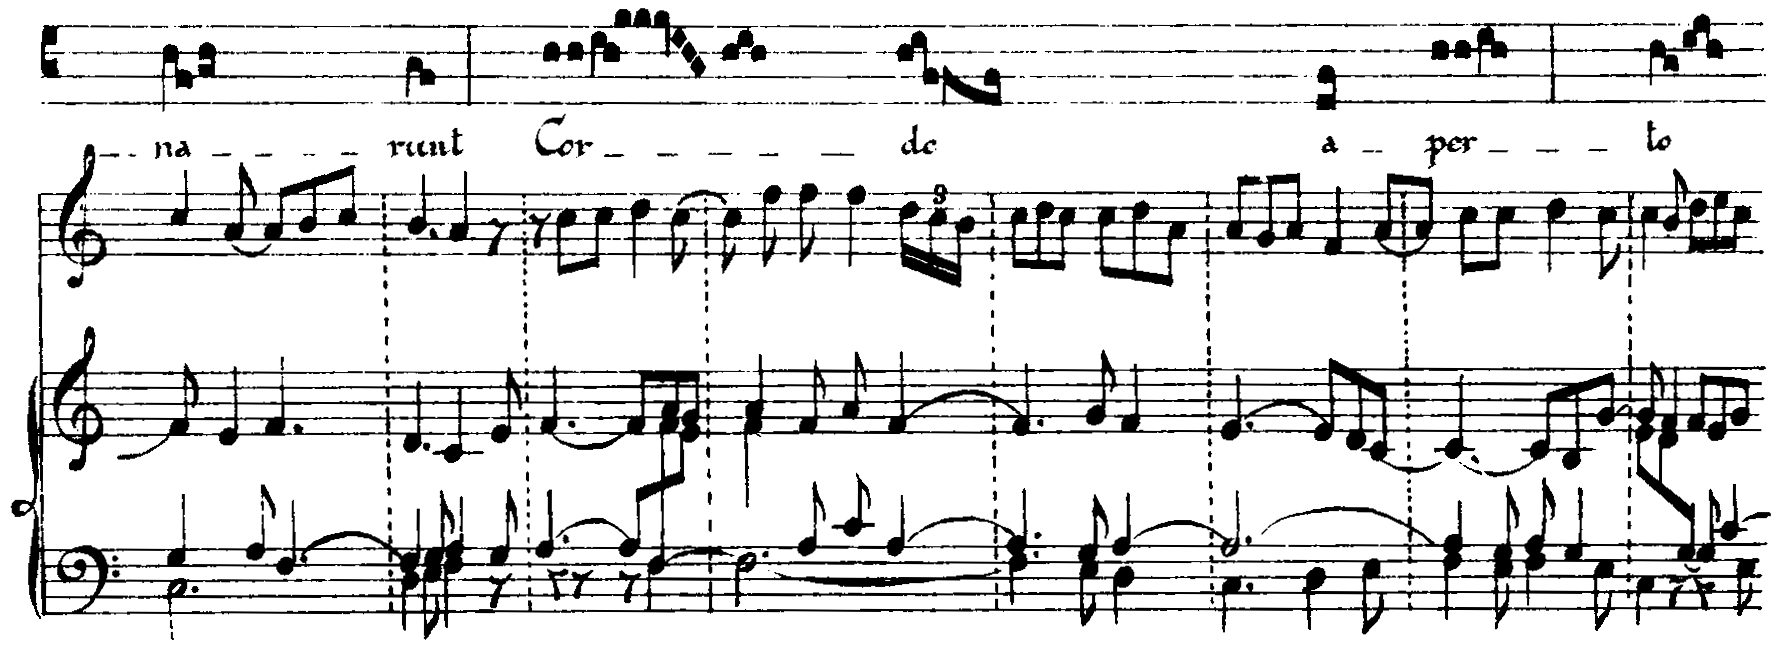
\includegraphics[width=\linewidth]{c/3/ex/bystrom_5_27.png}
  \caption{Byström, Mensural accompaniment barred in 6/8, 1892}
  \label{mus:bystrom_5_27}
\end{example}

\vspace*{\fill}

\clearpage

\vspace*{\fill}

\begin{example}
  \centering
  \includegraphics[width=.7\linewidth]{c/3/ex/processionale_1888_287.png}
  \caption{\emph{Processionale monasticum}, `Benedicta et venerabilis', 1888}
  \label{mus:processionale_1888_287}
\end{example}

\vspace*{\fill}

\begin{example}
  \centering
  \includegraphics[width=\linewidth]{c/3/ex/lhoumeau_benedicta_5_12.png}
  \caption{Lhoumeau, Accompaniment of \cref{mus:processionale_1888_287}, 1892}
  \label{mus:lhoumeau_benedicta_5_12}
\end{example}

\vspace*{\fill}

\clearpage

\vspace*{\fill}

\begin{example}
  \centering
  \includegraphics[width=.8\linewidth]{c/3/ex/lhoumeau_justus1.png}
  \\
  \includegraphics[width=.8\linewidth]{c/3/ex/lhoumeau_justus2.png}
  \\
  \includegraphics[width=.8\linewidth]{c/3/ex/lhoumeau_justus3.png}
  \\
  \includegraphics[width=.8\linewidth]{c/3/ex/lhoumeau_justus4.png}
  \caption{Lhoumeau, Alleluia \emph{Justus germinabit}, 1893}
  \label{mus:lhoumeau_justus}
\end{example}

\vspace*{\fill}

\begin{example}
  \centering
  \includegraphics[width=.8\linewidth]{c/3/ex/lhoumeau_douze1.png}
  \\
  \includegraphics[width=.8\linewidth]{c/3/ex/lhoumeau_douze2.png}
  \caption{Lhoumeau, Alleluia \emph{Fac nos innocuam}, 1893}
  \label{mus:lhoumeau_facnos}
\end{example}

\vspace*{\fill}

\clearpage

\begin{landscape}

  \vspace*{\fill}

  \begin{example}
    \centering
    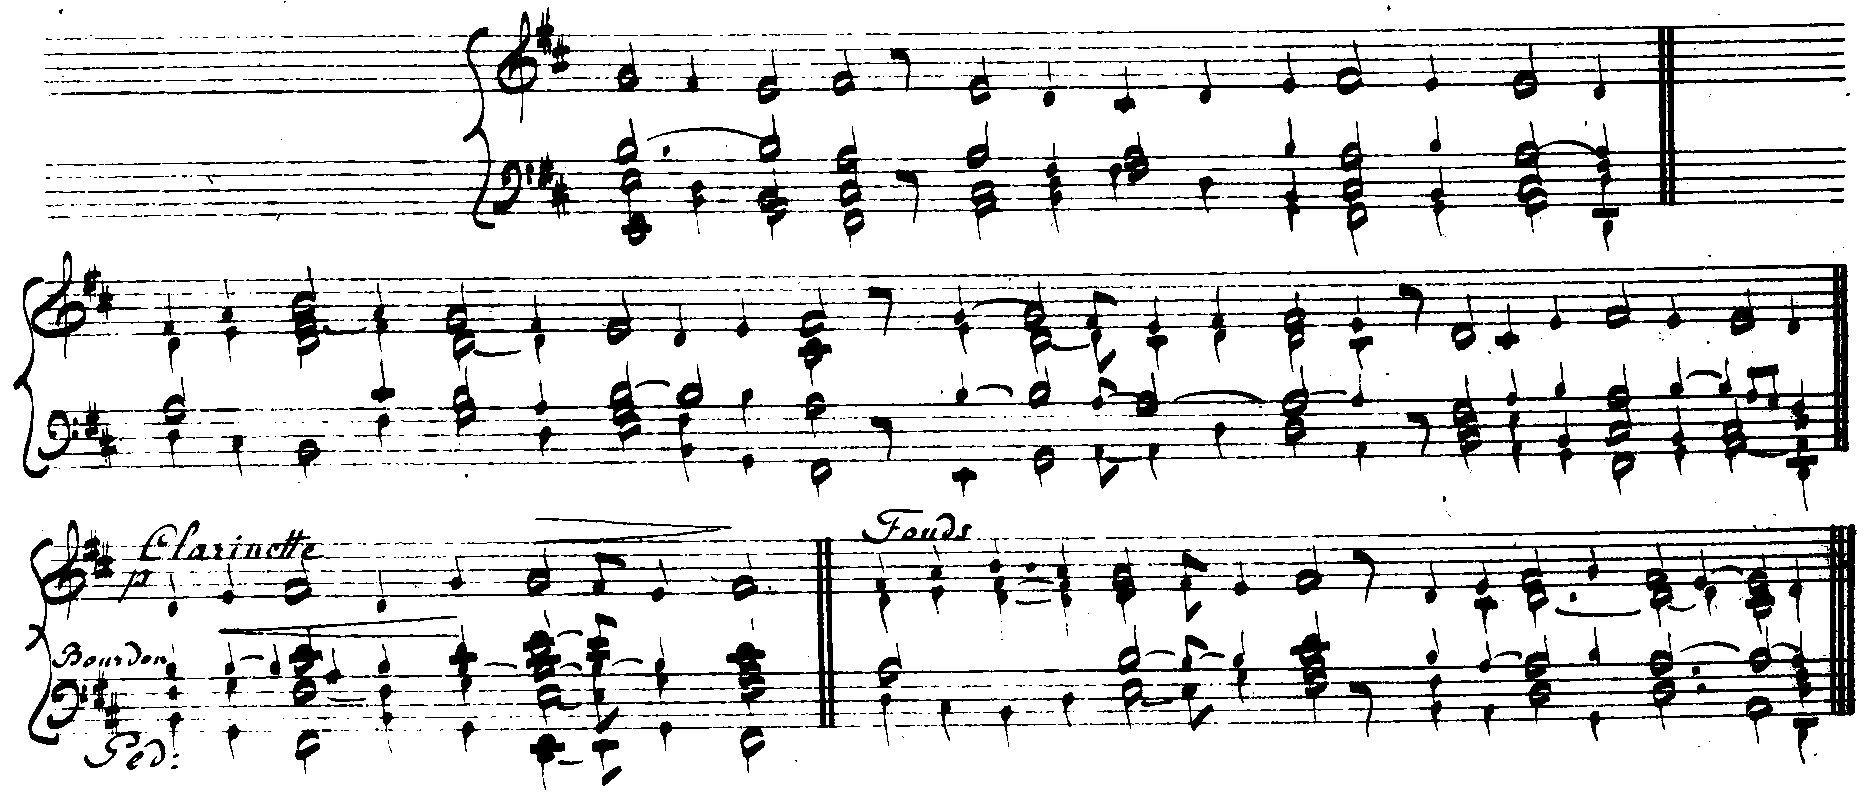
\includegraphics[width=\linewidth]{c/3/ex/guilmant_6979_1v.png}
    \caption{Guilmant, \bnf{} MS~6979, f.~1v}
    \label{mus:guilmant_6979_1v}
  \end{example}

  \vspace*{\fill}

  \clearpage

  \vspace*{\fill}

  \begin{example}
    \centering
    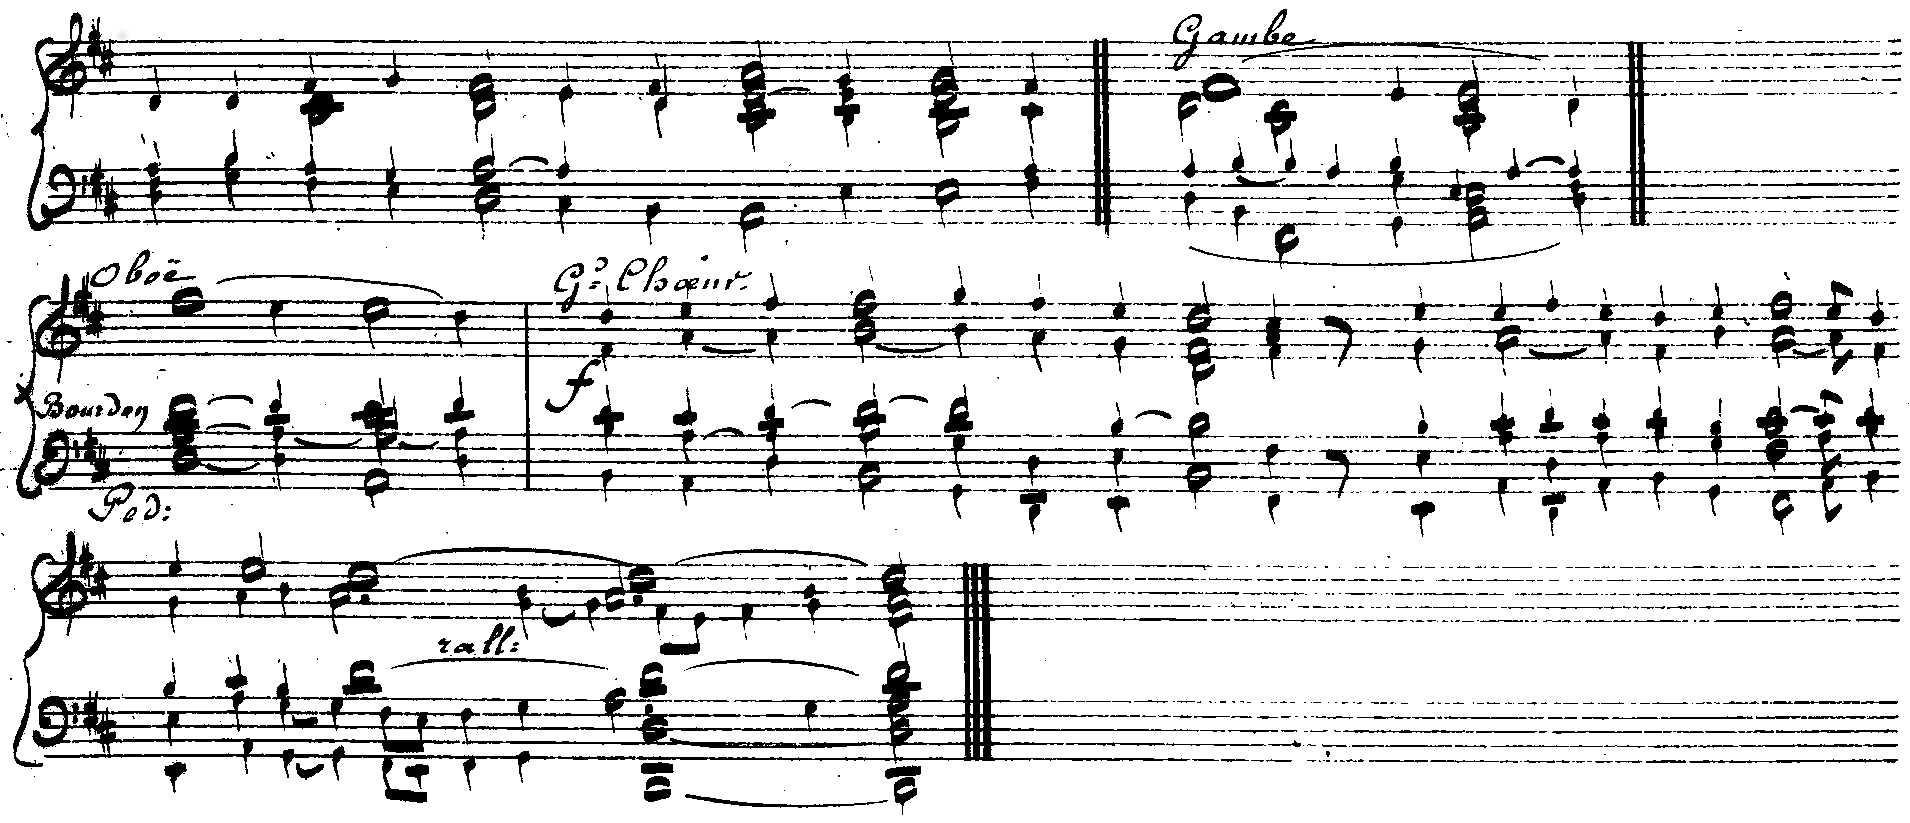
\includegraphics[width=\linewidth]{c/3/ex/guilmant_6979.png}
    \caption{Guilmant, \bnf{} MS~6979, f.~2r}
    \label{mus:guilmant_6979}
  \end{example}

\vspace*{\fill}

\end{landscape}

\vspace*{\fill}

\begin{example}
  \centering
  \includegraphics[width=\linewidth]{c/3/ex/guilmant_media_15.jpg}
  \caption{Guilmant, `Media vita', 1891}
  \label{mus:guilmant_media_15}
\end{example}

\vspace*{\fill}

\begin{example}
  \centering
  \includegraphics[width=\linewidth]{c/3/ex/tournemire_alleluiatique_9.png}
  \caption{Tournemire, `Choral alleluiatique \textnumero{} 2' from \emph{L'orgue mystique}, 1927--32}
  \label{mus:tournemire_alleluiatique_9}
\end{example}

\vspace*{\fill}


\clearpage
